\section{Target Audience \& Stakeholders}

While the previous sections established the technical and ergonomic landscape of wearable input devices, the viability of a glove-based air mouse depends entirely on its alignment with specific human needs and market realities. This section identifies the priority audiences and stakeholder-relevant user profiles for the proposed system, moving beyond general utility to define concrete adoption segments.

\subsection{Target Audience Segments and Adoption Rationale}

The broadest segment is the population of everyday technology users who are already comfortable with computers and Bluetooth peripherals but seek better ergonomics, mobility, or interaction novelty than conventional desk-bound mice. For this group, value is primarily practical: they need stable cursor response, low-friction pairing, and battery endurance sufficient for routine sessions in flexible contexts such as standing desks, couch/bed use, and ad hoc workspaces where a flat surface is inconvenient. This segment is strategically important because it provides the largest baseline adoption pool and the fastest path to real-world usage feedback.

The market scale for this segment is substantial. Recent market estimates place global PC users at approximately 1.86 billion, with continued annual growth in the low single-digit range~\cite{explodingtopics_pc_users_2024}. Even conservative conversion rates in such a base represent a meaningful opportunity for alternative input peripherals. Ergonomic burden within general computer users further supports this relevance: a Swedish population-oriented report indicates that musculoskeletal discomfort during computer work is common even among users without formal diagnosis, reinforcing that demand for alternatives is not limited to clinical populations~\cite{arbetsmiljoverket_workrelated_disorders_2024}. Occupational burden data from labor surveillance similarly indicate that repetitive-trauma exposure remains a major source of upper-limb injury and illness in modern work~\cite{bls_iif_2024}.

A second, high-priority segment is users with physical disability, reduced dexterity, or repetitive strain injury (RSI), including users affected by carpal tunnel syndrome (CTS), arthritis-related pain, post-stroke weakness, or persistent wrist/forearm overuse. For this segment, the glove is not merely a convenience accessory; it is an accessibility intervention. Surface-free interaction removes wrist-on-desk pressure, and threshold-based gesture logic can be tuned for reduced grip strength or constrained range of motion. This is especially relevant when commercial assistive alternatives are costly or offer limited customization.

Clinical and occupational evidence supports this priority. U.S. injury surveillance reports large annual burdens of work-related musculoskeletal injury and repetitive-trauma outcomes~\cite{bls_iif_2024,cdc_ergonomics_2024}. In the computer-using population specifically, prior evidence already included in this dissertation documents elevated CTS prevalence and strong exposure links in mouse-intensive work~\cite{dale2013cts,andersen2003mouse,thomsen2008mouse}. Broader accessibility evidence also supports the segment's strategic importance: people with disability remain under-served in digital access and device ownership, which implies a continuing need for adaptable and affordable interaction alternatives~\cite{perrin2021disabilitytech,duplaga2017disability}. From a product perspective, this segment also imposes the most stringent design constraints, making it a strong anchor for requirement quality.

A third high-value segment is presenters and educators, particularly in hybrid teaching and meeting environments where users need to move freely while maintaining control over slides, pointer movement, media playback, and annotation. The core behavioral pattern already exists in this market through wireless clickers and presenter remotes. The glove proposition is therefore not behavioral replacement, but functional expansion: one wearable controller for both navigation and full cursor interaction. Market analyses report sustained growth in wireless presentation-controller categories and related interactive classroom ecosystems, indicating stable demand for presentation mobility tools~\cite{wiredclicker_market_2024,verifiedmarketreports_clicker_2023}.

A fourth segment is gamers and VR/AR enthusiasts, where perceived immersion and expressive control can motivate early experimentation with unconventional input hardware. This segment is performance-sensitive and therefore acts as a stress test for latency, fusion stability, and gesture reliability. Global gaming participation and PC gaming market size remain extremely large, while enthusiast communities are often receptive to customizable open-source hardware and firmware workflows~\cite{newzoo_gaming_2024,steam_concurrent_2025}. For this audience, the glove concept is attractive only if end-to-end delay and aiming stability approach competitive usability thresholds.

Taken together, these segments define a clear prioritization strategy. Everyday users provide scale, disability/RSI users provide the strongest social and accessibility impact, presenters/educators provide immediate workflow fit, and gaming communities provide performance-driven refinement pressure. This multi-segment structure improves deployment realism by balancing market size, inclusion value, and technical rigor.

\subsection{Representative Use Cases and Persona-Driven Requirements}

Use-case analysis translates segment-level assumptions into concrete interaction scenarios. In rehabilitation-oriented home or clinic settings, a user recovering from stroke may have partial hand movement but difficulty gripping or sliding a traditional mouse. In this scenario, low-amplitude wrist rotation combined with simple finger gestures can restore core digital independence for browsing, communication, and form completion. In education settings, a lecturer can move between board and audience while controlling slides and cursor without returning to a desk device. In advanced productivity or gaming contexts, users can combine one-hand gestural pointing with keyboard shortcuts for command-dense workflows.

To operationalize these scenarios, this chapter introduces a representative persona: \textbf{Marco R.}, a 34-year-old freelance graphic designer based in Valencia who works remotely and spends 6--10 hours daily on design tools. Marco has a history of CTS-related pain, has already tested vertical and trackball devices with only partial relief, and requires high cursor precision for visual editing tasks. His central constraint is not basic computer literacy but sustained usability under pain and fatigue. This profile is strategically useful because it combines high precision demand, prolonged exposure, moderate technical confidence, and strong motivation to adopt alternatives if setup friction is low.

Marco's requirement profile is practical and measurable: zero wrist-to-surface contact, precision sufficient for design software, adjustable sensitivity without firmware editing, battery life above one extended session, and reliable Bluetooth pairing on mainstream desktop platforms. His pain points include recurring daily discomfort with conventional mice, high prices for specialized assistive devices, and inability to self-maintain code-level settings during active work. In product terms, this implies that usability depends as much on onboarding and stability as on raw sensing quality.

Figure~\ref{fig:ch5_persona_profile} summarizes this persona using normalized usage and constraint indicators derived from the provided profile. The figure is intended as a requirement communication artifact: it visually prioritizes what must be optimized first during prototype maturation.

\begin{figure}[H]
  \centering
  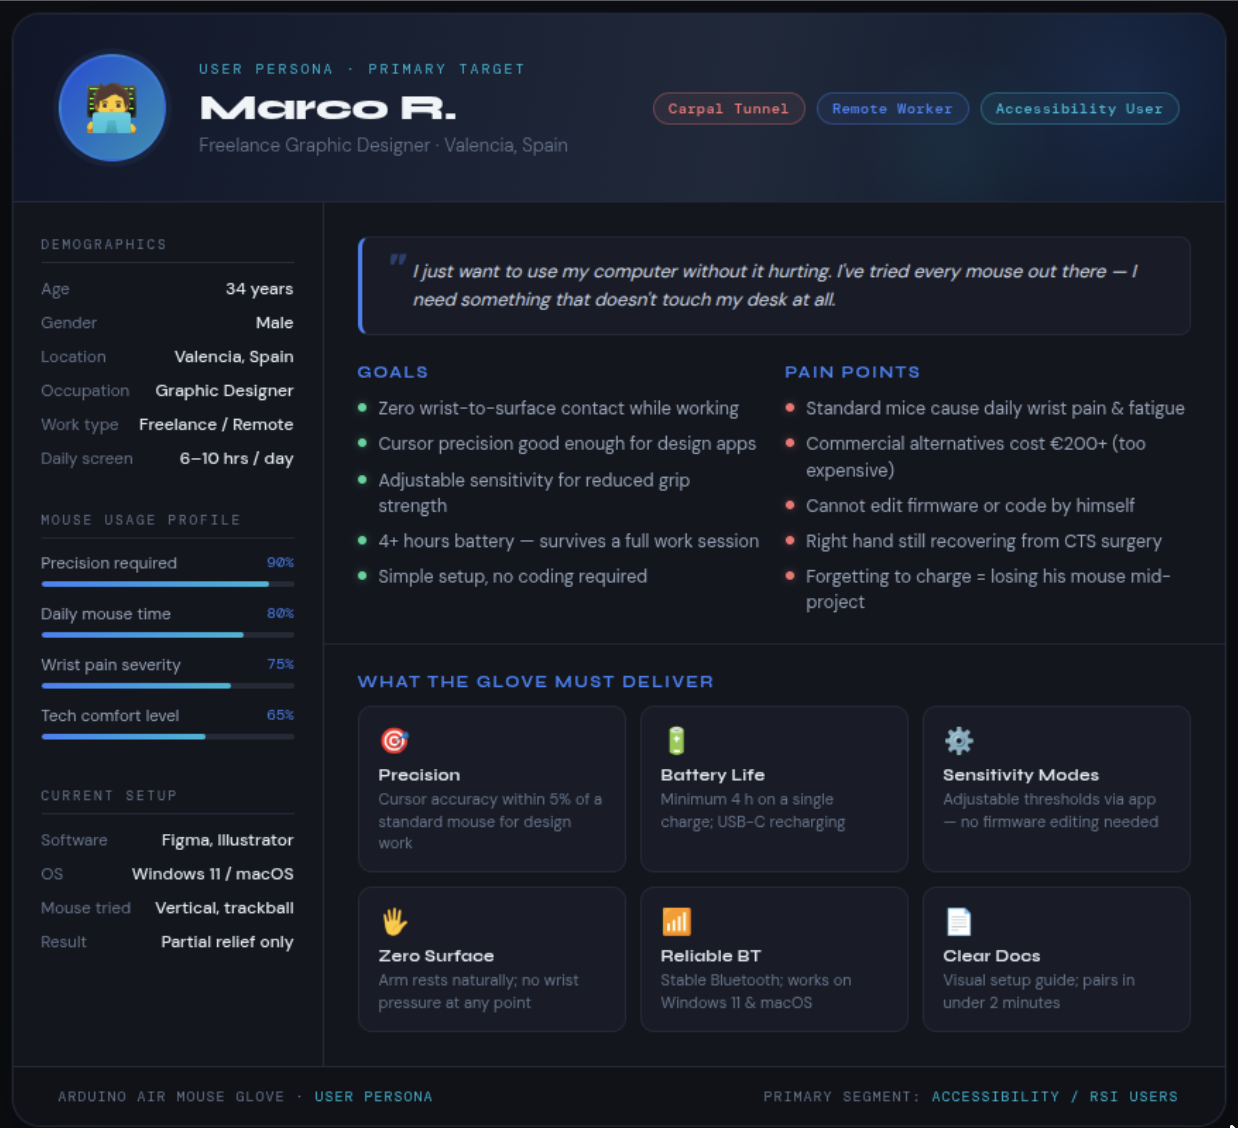
\includegraphics[width=0.6\linewidth]{img/1.png}
  \caption{User Persona Profile for a High-Precision Remote Worker in CTS Recovery}
  \label{fig:ch5_persona_profile}
\end{figure}

Interpreted together, the use cases and persona data provide direct engineering direction. Cursor behavior must remain stable during low-amplitude motion, click actions must avoid accidental displacement, pairing and reconnection must be predictable, and energy management must cover uninterrupted work sessions. These are not optional quality features: they are minimum viability conditions for the most meaningful target users.

\subsection{User Validation \& Statistical Analysis}

The following analysis based on $N=100$ respondents validates the core hypothesis: there is a clear demand for a wearable, gesture-based peripheral, particularly for specialized professional and ergonomic use cases.

% --- DISCOMFORT ANALYSIS ---
\subsubsection{Ergonomic Pain Points}
\begin{figure}[H]
    \centering
    \begin{tikzpicture}
        \pie[rotate=90, text=pin, radius=2.0, color={blue!60, cyan!40, orange!60, red!60, gray!40}]{
            25/Never, 35/Rarely, 20/Sometimes, 15/Often, 5/Always
        }
    \end{tikzpicture}
    \caption{Frequency of Mouse-Related Discomfort}
\end{figure}

\textbf{Analysis:} Over \textbf{40\% of users} report experiencing discomfort "Sometimes" to "Always," while only 25\% report "Never." This distribution confirms that wrist-strain risk is not a marginal issue but a mainstream usability constraint. The ergonomic value proposition should therefore be framed as \textit{pain prevention and fatigue reduction}, not only as interaction novelty. In practical terms, this supports prioritising low-force click gestures, drift-resistant pointer behaviour during micro-movements, and calibration modes for users with reduced range of motion.

% --- USE CASE ANALYSIS ---
\subsubsection{Market Segmentation and Use Cases}

\begin{figure}[H]
    \centering
    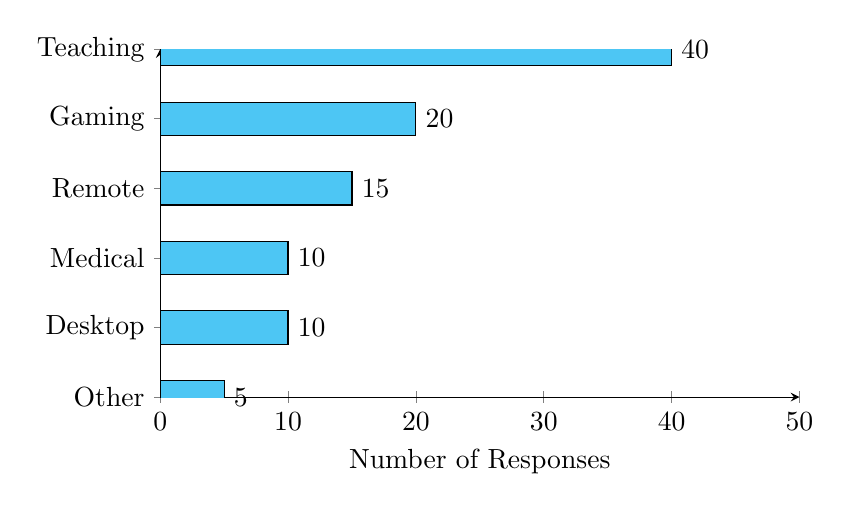
\begin{tikzpicture}
        \begin{axis}[
            xbar, xmin=0, xmax=50, width=0.8\textwidth, height=6cm,
            xlabel={Number of Responses},
            symbolic y coords={{Other}, {Desktop}, {Medical}, {Remote}, {Gaming}, {Teaching}},
            ytick=data, nodes near coords, nodes near coords align={horizontal},
            axis x line=bottom, axis y line=left, bar width=12pt
        ]
            \addplot[fill=cyan!70] coordinates {(40,{Teaching}) (20,{Gaming}) (15,{Remote}) (10,{Medical}) (10,{Desktop}) (5,{Other})};
        \end{axis}
    \end{tikzpicture}
    \caption{Primary Use Case Validation}
\end{figure}

The data identifies \textbf{Presentations and Teaching (40\%)} as the primary entry market, followed by Gaming (20\%) and Remote Work (15\%). This indicates that \textit{mobility-centric contexts} dominate early adoption intent: users value standing movement, room-scale interaction, and cursor control away from a fixed desk. Strategically, this supports a phased go-to-market model: first optimise presenter-grade reliability (slide navigation, stable cursor, rapid reconnect), then expand toward precision-demand segments such as design-heavy remote work and gaming. The chart therefore justifies a "Pro-Presenter first, precision expansion second" product trajectory rather than immediate mass-market desktop replacement.



% --- BARRIERS & ADOPTION ---
\subsubsection{Adoption Likelihood vs. Technical Barriers}
\begin{figure}[H]
    \centering
    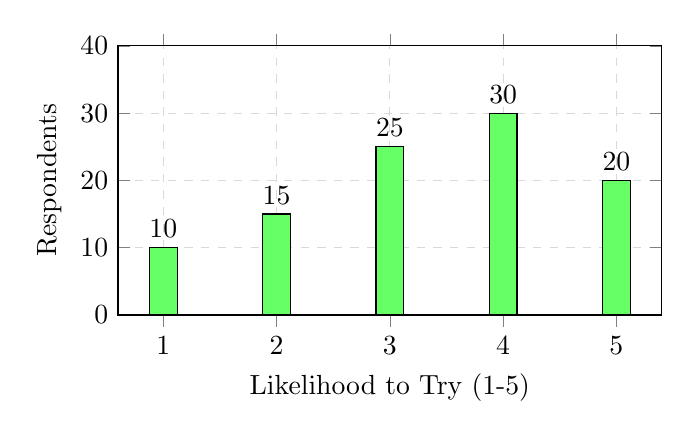
\begin{tikzpicture}
        \begin{axis}[
            ybar, ymin=0, ymax=40, width=0.7\textwidth, height=5cm,
            ylabel={Respondents}, xlabel={Likelihood to Try (1-5)},
            xtick=data, symbolic x coords={1, 2, 3, 4, 5},
            nodes near coords, grid=major, grid style={dashed, gray!30}
        ]
            \addplot[fill=green!60] coordinates {(1,10) (2,15) (3,25) (4,30) (5,20)};
        \end{axis}
    \end{tikzpicture}
    \caption{Consumer Interest Distribution}
\end{figure}

\textbf{Analysis:} With \textbf{50\% of respondents} scoring 4 or 5, baseline willingness to trial is strong; however, the central adoption signal is \textit{conditional enthusiasm}. Users are interested, but conversion depends on two gatekeepers: cost (30\%) and perceived precision (25\%). This implies that technical maturity and affordability must progress together. From an engineering perspective, the prototype should transition from exploratory sensing to a higher-stability IMU pipeline with improved filtering, repeatable calibration, and quantifiable jitter control. From a product perspective, bill-of-material choices should be evaluated against a target entry price band so that performance gains are not negated by cost-driven drop-off.





\subsection{Stakeholders}

Beyond direct users, the present work involves stakeholders who influence adoption, validation, and long-term viability. Population-level digital access disparities reinforce this broader relevance: adults with disabilities report lower computer ownership (62\% versus 81\%) and higher rates of never going online (15\% versus 5\%) than adults without disabilities~\cite{perrin2021disabilitytech}. Similar disparities are reported in non-US settings, including substantially lower internet participation among respondents with disabilities in Poland~\cite{duplaga2017disability}. At organisational level, the stakeholder case is also economic: musculoskeletal disorders have been associated with major direct and indirect occupational costs~\cite{nrc2001msd}, while WHO/ILO estimates indicate sustained growth in work-related musculoskeletal burden over time~\cite{whoilo2021wrmsd}. Appendix Table~\ref{tbl:stakeholders_appendix} summarises the main groups, their interests, and the evidence supporting their relevance.
\begin{figure}[H]
\centering
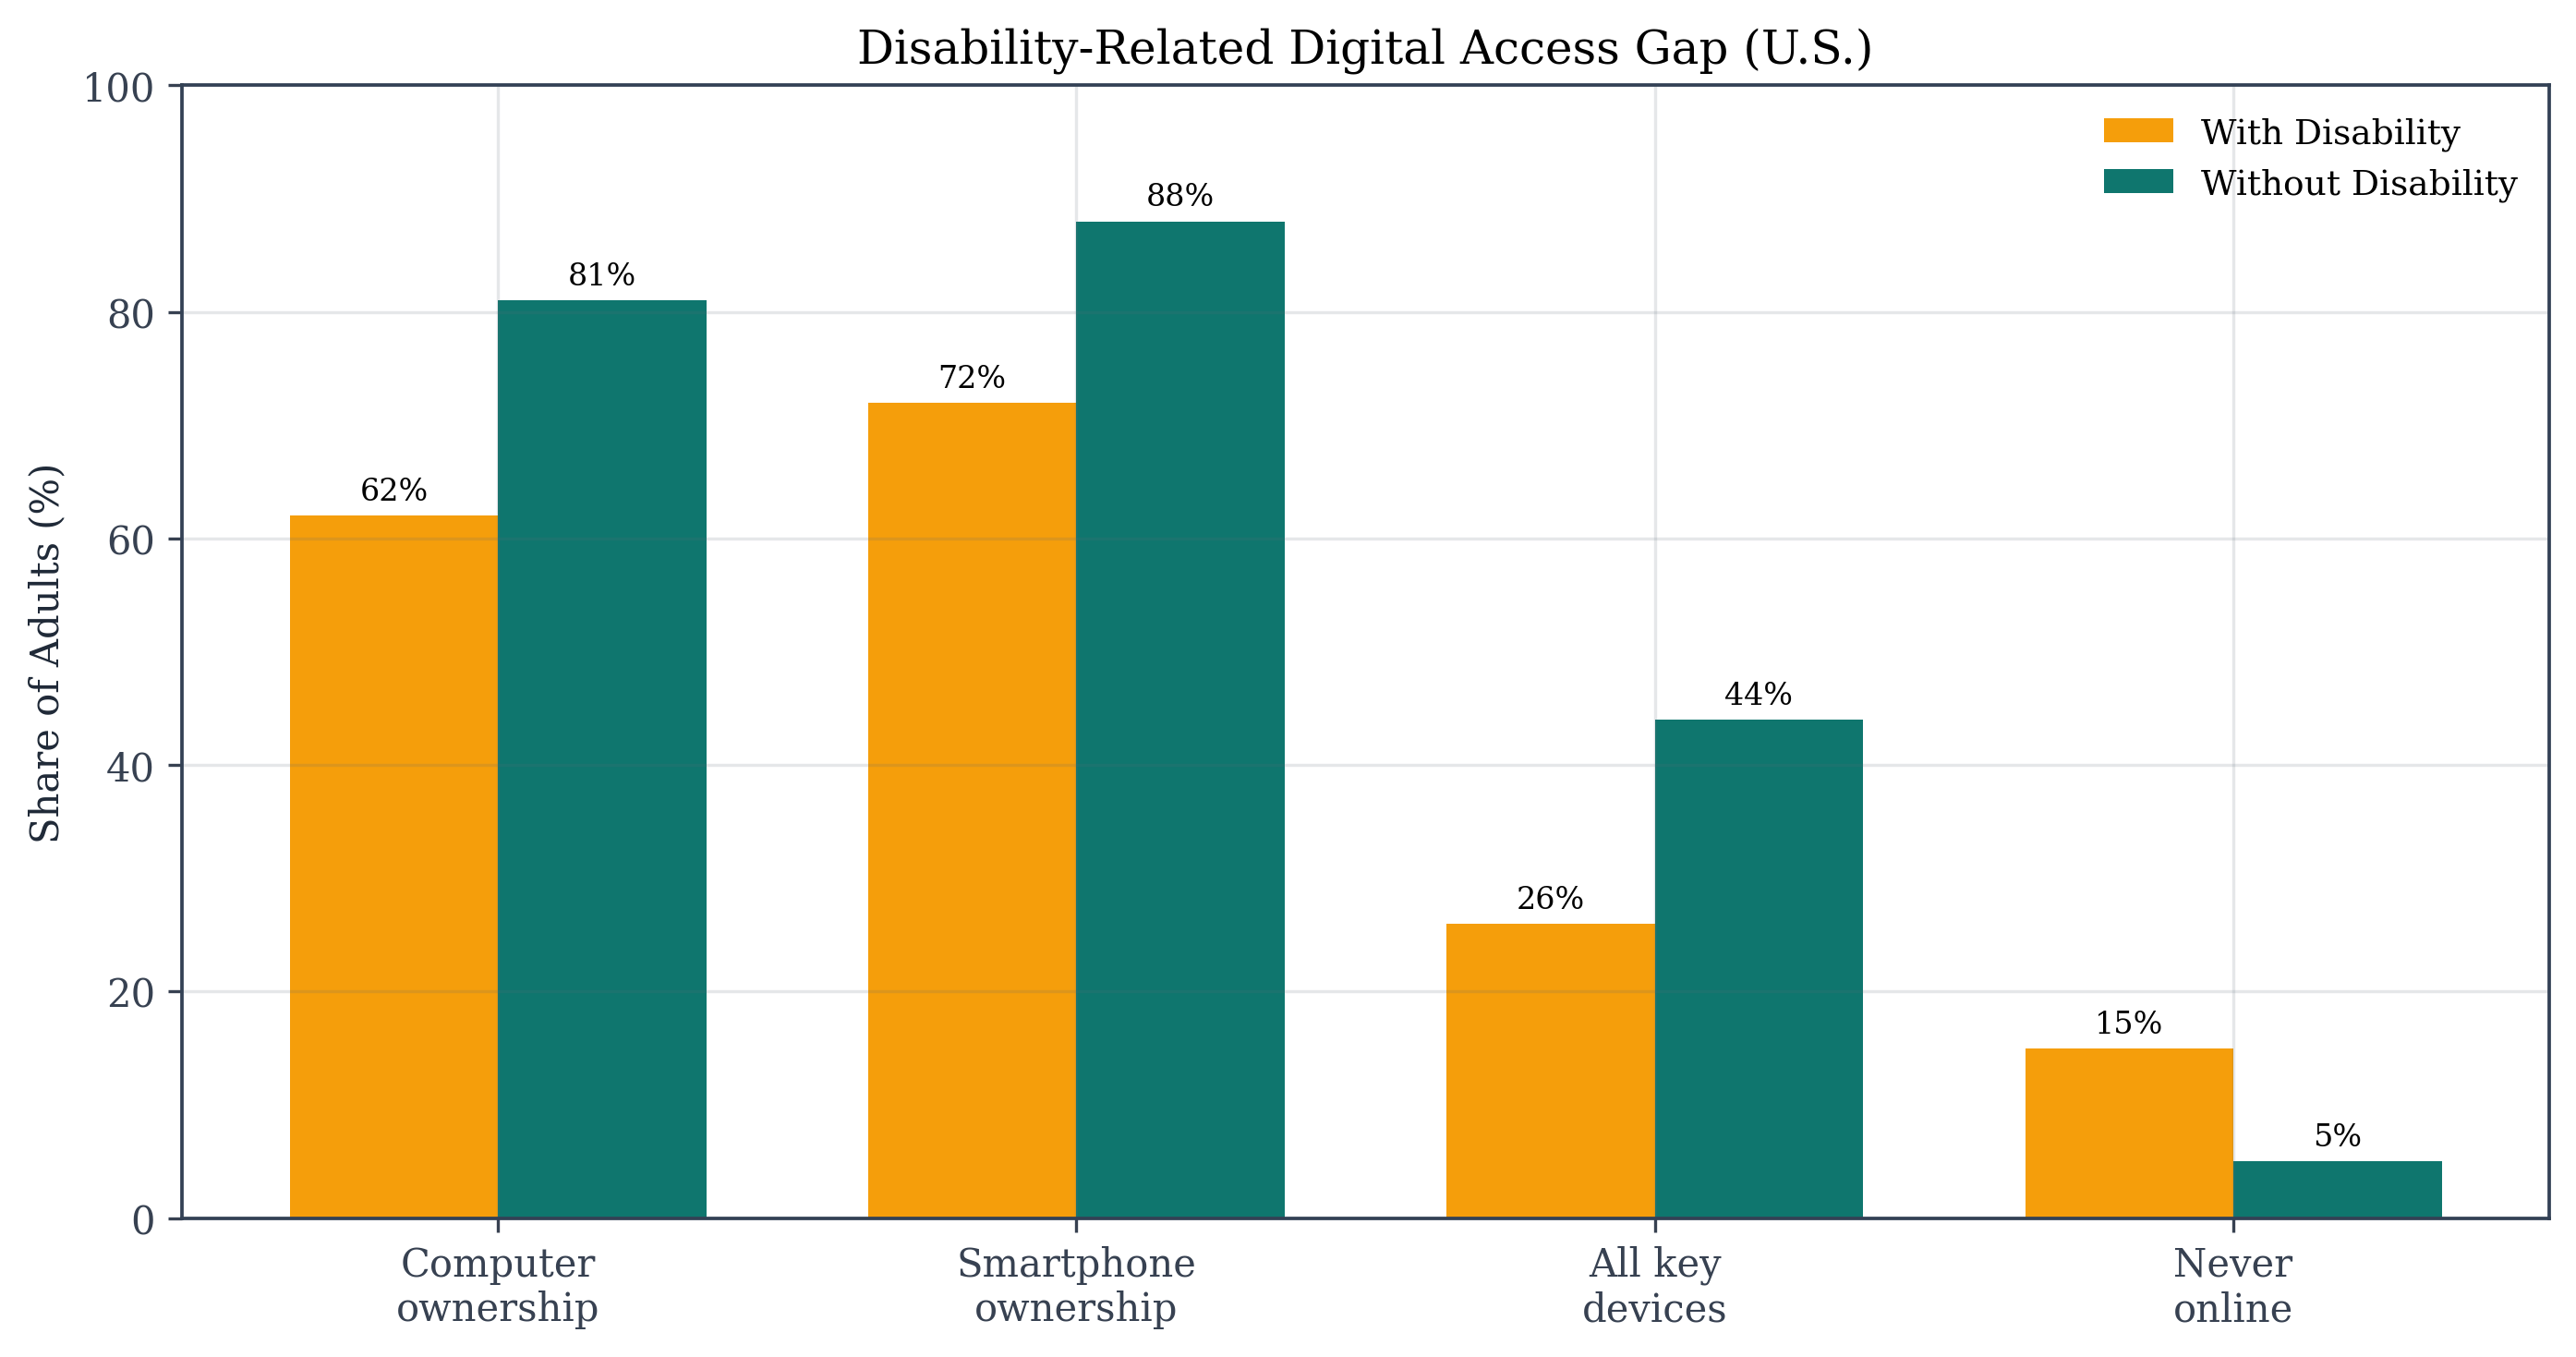
\includegraphics[width=0.75\linewidth]{img/ch5_disability_digital_divide.png}
\caption{Disability-Related Digital Access Gap in U.S. Survey Data}
\label{fig:digital_divide_stakeholder}
\end{figure}
Figure~\ref{fig:digital_divide_stakeholder} visualises the digital-access asymmetry that motivates stakeholder involvement beyond direct end users, particularly for institutions responsible for equitable deployment.



For stakeholder analysis, this pattern indicates that accessibility constraints are not isolated edge cases but population-level participation constraints. Consequently, institutional stakeholders are relevant not only for procurement and deployment but also for inclusion outcomes.

The detailed stakeholder matrix is provided in Appendix Table~\ref{tbl:stakeholders_appendix}.



The table operationalises stakeholder prioritisation by linking each group to a concrete validation signal, which supports transparent evaluation criteria in later chapters.

\subsection{Design Implications, Stakeholder Fit, and Validation Priorities}

The target-audience analysis creates a concrete bridge between user diversity and implementation planning. For everyday users, success depends on simplicity and perceived reliability: fast setup, robust Bluetooth behavior, and low-maintenance operation. For disability and RSI populations, success depends on tunable sensitivity, low-force interaction, and repeatable control under motor variability. For presenters and educators, success depends on mobility without control interruption. For gamers and enthusiasts, success depends on latency discipline and response consistency under high interaction frequency. 

These requirements also map cleanly to stakeholder interests discussed in earlier chapters. Accessibility practitioners and rehabilitation professionals can evaluate personalization benefit. Educational institutions can evaluate deployment in teaching environments. Employers and occupational-health stakeholders can evaluate ergonomic sustainability in high-exposure computer workflows. Open-source contributors can iterate sensing and interaction logic using transparent firmware pathways. This alignment is important because it increases the probability of adoption beyond single-user prototypes.




